%% fig_bypass.tex   (generated by make_frontier.py; do not edit by hand)
%% The ten routes to the Mumford target that avoid the Lefschetz standard conjecture, with the status of each.
\documentclass[tikz,border=6pt]{standalone}
\usepackage{amsmath,amssymb}
\usetikzlibrary{arrows.meta,calc,decorations.pathreplacing,patterns}
%% palette.tex -- shared colour definitions for the figures
\definecolor{PInk}{RGB}{26,32,44}
\definecolor{PBlue}{RGB}{37,82,139}
\definecolor{PTeal}{RGB}{23,127,125}
\definecolor{POchre}{RGB}{193,138,44}
\definecolor{PClay}{RGB}{178,74,58}
\definecolor{PSlate}{RGB}{108,122,137}
\definecolor{PViolet}{RGB}{110,86,150}
\definecolor{WBlue}{RGB}{223,234,246}
\definecolor{WTeal}{RGB}{220,238,236}
\definecolor{WOchre}{RGB}{250,240,218}
\definecolor{WClay}{RGB}{247,229,224}
\definecolor{WSlate}{RGB}{238,241,244}
\definecolor{PMag}{RGB}{158,58,110}
\definecolor{PGrass}{RGB}{62,124,66}
\definecolor{PAmber}{RGB}{214,112,38}
\definecolor{PIndigo}{RGB}{58,64,140}
\definecolor{PRule}{RGB}{176,186,197}

%% shared macros so the standalone figures match the paper
\providecommand{\QQ}{\mathbb{Q}}
\providecommand{\ZZ}{\mathbb{Z}}
\providecommand{\RR}{\mathbb{R}}
\providecommand{\CC}{\mathbb{C}}
\providecommand{\PP}{\mathbb{P}}
\providecommand{\Kx}{K^{\times}}
\providecommand{\HW}{W}
\providecommand{\Nm}{\mathrm{N}}
\providecommand{\Hdg}{\mathrm{Hdg}}
\providecommand{\NS}{\mathrm{NS}}
\providecommand{\cA}{\mathcal{A}}
\providecommand{\cD}{\mathcal{D}}
\providecommand{\cF}{\mathcal{F}}
\providecommand{\cP}{\mathcal{P}}
\providecommand{\cO}{\mathcal{O}}
\providecommand{\cQ}{\mathcal{Q}}
\providecommand{\bbar}[1]{\overline{#1}}
\providecommand{\ch}{\operatorname{ch}}
\providecommand{\End}{\mathrm{End}}
\providecommand{\Ext}{\operatorname{Ext}}
\providecommand{\Supp}{\operatorname{Supp}}

\begin{document}
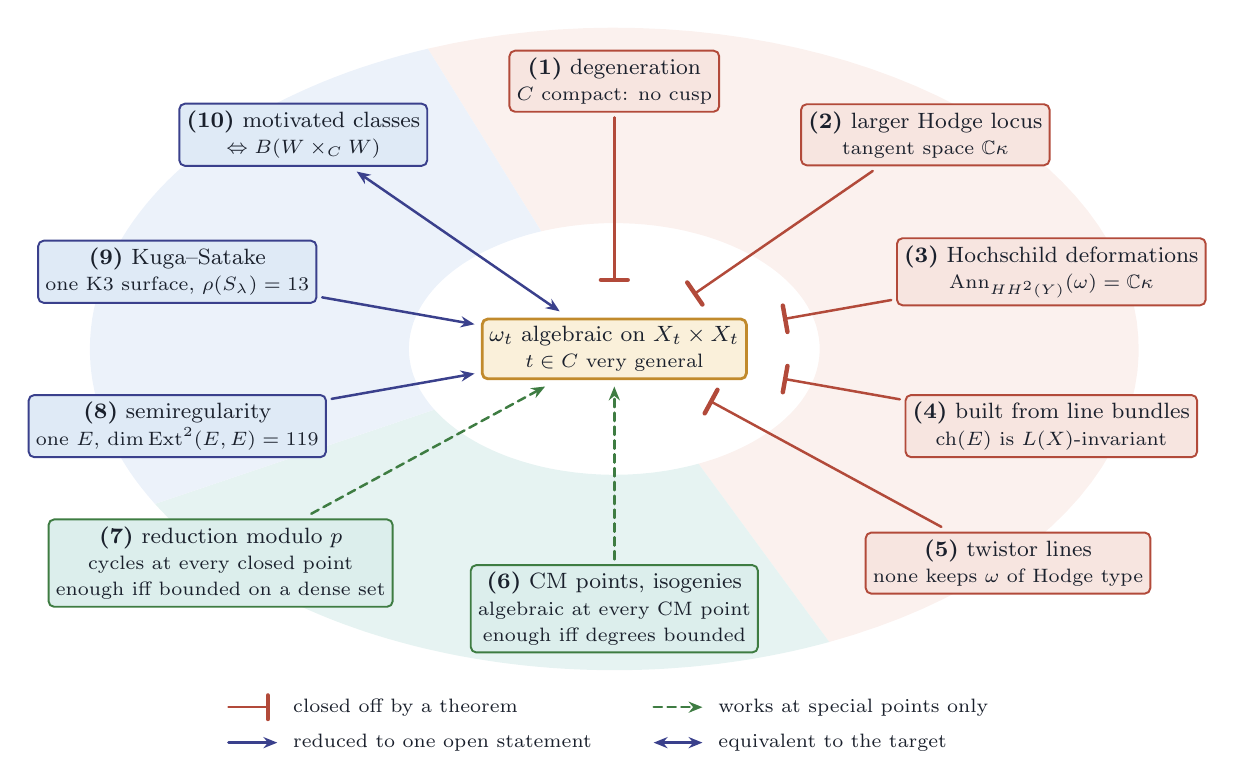
\begin{tikzpicture}[x=1cm,y=1cm,line join=round,line cap=round,
  font=\small,text=PInk]
  \fill[WClay!55] (-2.368,3.813) -- (-2.045,3.883) -- (-1.717,3.942) -- (-1.384,3.991) -- (-1.048,4.029) -- (-0.709,4.057) -- (-0.368,4.074) -- (-0.026,4.080) -- (0.316,4.075) -- (0.658,4.060) -- (0.997,4.034) -- (1.334,3.997) -- (1.667,3.950) -- (1.996,3.892) -- (2.320,3.824) -- (2.637,3.746) -- (2.948,3.659) -- (3.251,3.561) -- (3.545,3.454) -- (3.830,3.338) -- (4.105,3.213) -- (4.369,3.080) -- (4.621,2.938) -- (4.861,2.789) -- (5.089,2.632) -- (5.303,2.469) -- (5.503,2.299) -- (5.688,2.122) -- (5.858,1.941) -- (6.013,1.754) -- (6.152,1.562) -- (6.275,1.367) -- (6.382,1.167) -- (6.471,0.965) -- (6.543,0.760) -- (6.598,0.553) -- (6.636,0.345) -- (6.656,0.136) -- (6.659,-0.074) -- (6.644,-0.283) -- (6.611,-0.492) -- (6.561,-0.699) -- (6.494,-0.905) -- (6.410,-1.108) -- (6.308,-1.308) -- (6.190,-1.505) -- (6.056,-1.698) -- (5.906,-1.886) -- (5.740,-2.069) -- (5.559,-2.247) -- (5.363,-2.419) -- (5.153,-2.585) -- (4.930,-2.743) -- (4.693,-2.895) -- (4.444,-3.039) -- (4.184,-3.174) -- (3.912,-3.302) -- (3.630,-3.421) -- (3.339,-3.530) -- (3.038,-3.631) -- (2.730,-3.722) -- (1.069,-1.458) -- (1.190,-1.422) -- (1.308,-1.383) -- (1.422,-1.340) -- (1.532,-1.293) -- (1.639,-1.243) -- (1.741,-1.190) -- (1.838,-1.134) -- (1.931,-1.074) -- (2.018,-1.012) -- (2.101,-0.947) -- (2.177,-0.880) -- (2.248,-0.810) -- (2.313,-0.739) -- (2.372,-0.665) -- (2.425,-0.589) -- (2.471,-0.512) -- (2.510,-0.434) -- (2.544,-0.354) -- (2.570,-0.274) -- (2.589,-0.193) -- (2.602,-0.111) -- (2.608,-0.029) -- (2.607,0.053) -- (2.599,0.135) -- (2.584,0.217) -- (2.563,0.298) -- (2.534,0.378) -- (2.499,0.457) -- (2.458,0.535) -- (2.410,0.612) -- (2.355,0.687) -- (2.295,0.760) -- (2.228,0.831) -- (2.155,0.900) -- (2.077,0.967) -- (1.993,1.031) -- (1.904,1.092) -- (1.810,1.151) -- (1.711,1.206) -- (1.608,1.258) -- (1.500,1.307) -- (1.388,1.353) -- (1.273,1.395) -- (1.155,1.433) -- (1.033,1.467) -- (0.909,1.498) -- (0.782,1.525) -- (0.653,1.547) -- (0.522,1.566) -- (0.391,1.580) -- (0.258,1.590) -- (0.124,1.596) -- (-0.010,1.598) -- (-0.144,1.596) -- (-0.278,1.589) -- (-0.410,1.578) -- (-0.542,1.563) -- (-0.673,1.544) -- (-0.801,1.521) -- (-0.928,1.494) -- cycle;
  \fill[WTeal!70] (2.730,-3.722) -- (2.578,-3.762) -- (2.425,-3.800) -- (2.270,-3.836) -- (2.114,-3.869) -- (1.957,-3.900) -- (1.798,-3.929) -- (1.638,-3.955) -- (1.477,-3.978) -- (1.316,-4.000) -- (1.153,-4.018) -- (0.990,-4.035) -- (0.826,-4.048) -- (0.662,-4.060) -- (0.497,-4.069) -- (0.332,-4.075) -- (0.167,-4.079) -- (0.002,-4.080) -- (-0.164,-4.079) -- (-0.329,-4.075) -- (-0.494,-4.069) -- (-0.659,-4.060) -- (-0.823,-4.049) -- (-0.987,-4.035) -- (-1.150,-4.019) -- (-1.313,-4.000) -- (-1.474,-3.979) -- (-1.635,-3.955) -- (-1.795,-3.929) -- (-1.954,-3.901) -- (-2.111,-3.870) -- (-2.267,-3.836) -- (-2.422,-3.801) -- (-2.575,-3.763) -- (-2.727,-3.722) -- (-2.877,-3.680) -- (-3.025,-3.635) -- (-3.172,-3.588) -- (-3.316,-3.538) -- (-3.458,-3.487) -- (-3.599,-3.433) -- (-3.737,-3.377) -- (-3.872,-3.319) -- (-4.006,-3.260) -- (-4.137,-3.198) -- (-4.265,-3.134) -- (-4.391,-3.068) -- (-4.513,-3.000) -- (-4.634,-2.931) -- (-4.751,-2.859) -- (-4.865,-2.786) -- (-4.977,-2.711) -- (-5.085,-2.635) -- (-5.190,-2.557) -- (-5.292,-2.477) -- (-5.391,-2.396) -- (-5.487,-2.313) -- (-5.579,-2.229) -- (-5.667,-2.143) -- (-5.752,-2.056) -- (-5.834,-1.968) -- (-2.285,-0.771) -- (-2.253,-0.805) -- (-2.220,-0.839) -- (-2.185,-0.873) -- (-2.149,-0.906) -- (-2.112,-0.938) -- (-2.073,-0.970) -- (-2.033,-1.001) -- (-1.992,-1.032) -- (-1.949,-1.062) -- (-1.906,-1.091) -- (-1.861,-1.120) -- (-1.815,-1.148) -- (-1.768,-1.175) -- (-1.720,-1.202) -- (-1.670,-1.227) -- (-1.620,-1.252) -- (-1.569,-1.277) -- (-1.517,-1.300) -- (-1.464,-1.323) -- (-1.409,-1.345) -- (-1.355,-1.366) -- (-1.299,-1.386) -- (-1.242,-1.405) -- (-1.185,-1.424) -- (-1.127,-1.441) -- (-1.068,-1.458) -- (-1.009,-1.474) -- (-0.949,-1.489) -- (-0.888,-1.503) -- (-0.827,-1.516) -- (-0.765,-1.528) -- (-0.703,-1.539) -- (-0.640,-1.549) -- (-0.577,-1.558) -- (-0.514,-1.567) -- (-0.450,-1.574) -- (-0.387,-1.580) -- (-0.322,-1.586) -- (-0.258,-1.590) -- (-0.194,-1.594) -- (-0.129,-1.596) -- (-0.064,-1.598) -- (0.001,-1.598) -- (0.065,-1.597) -- (0.130,-1.596) -- (0.195,-1.594) -- (0.259,-1.590) -- (0.324,-1.586) -- (0.388,-1.580) -- (0.452,-1.574) -- (0.515,-1.567) -- (0.579,-1.558) -- (0.642,-1.549) -- (0.704,-1.539) -- (0.766,-1.527) -- (0.828,-1.515) -- (0.889,-1.502) -- (0.950,-1.488) -- (1.010,-1.473) -- (1.069,-1.458) -- cycle;
  \fill[WBlue!60] (-5.834,-1.968) -- (-5.923,-1.865) -- (-6.007,-1.761) -- (-6.087,-1.656) -- (-6.162,-1.549) -- (-6.231,-1.440) -- (-6.296,-1.331) -- (-6.355,-1.221) -- (-6.409,-1.109) -- (-6.458,-0.997) -- (-6.502,-0.884) -- (-6.540,-0.770) -- (-6.574,-0.655) -- (-6.601,-0.540) -- (-6.624,-0.425) -- (-6.641,-0.309) -- (-6.653,-0.193) -- (-6.659,-0.076) -- (-6.660,0.040) -- (-6.655,0.156) -- (-6.645,0.272) -- (-6.630,0.388) -- (-6.609,0.504) -- (-6.583,0.619) -- (-6.551,0.734) -- (-6.515,0.848) -- (-6.472,0.961) -- (-6.425,1.074) -- (-6.372,1.186) -- (-6.315,1.297) -- (-6.252,1.406) -- (-6.184,1.515) -- (-6.111,1.622) -- (-6.033,1.728) -- (-5.950,1.833) -- (-5.862,1.936) -- (-5.770,2.038) -- (-5.673,2.138) -- (-5.571,2.236) -- (-5.464,2.332) -- (-5.354,2.427) -- (-5.239,2.519) -- (-5.119,2.610) -- (-4.996,2.698) -- (-4.868,2.784) -- (-4.737,2.868) -- (-4.601,2.950) -- (-4.462,3.029) -- (-4.319,3.106) -- (-4.173,3.180) -- (-4.023,3.251) -- (-3.870,3.320) -- (-3.714,3.387) -- (-3.555,3.450) -- (-3.393,3.511) -- (-3.228,3.569) -- (-3.061,3.623) -- (-2.891,3.675) -- (-2.719,3.724) -- (-2.545,3.770) -- (-2.368,3.813) -- (-0.928,1.494) -- (-0.997,1.477) -- (-1.065,1.459) -- (-1.132,1.440) -- (-1.199,1.419) -- (-1.264,1.398) -- (-1.329,1.375) -- (-1.392,1.351) -- (-1.455,1.326) -- (-1.516,1.300) -- (-1.576,1.273) -- (-1.634,1.245) -- (-1.692,1.216) -- (-1.748,1.186) -- (-1.802,1.155) -- (-1.855,1.123) -- (-1.907,1.091) -- (-1.957,1.057) -- (-2.005,1.022) -- (-2.052,0.987) -- (-2.097,0.951) -- (-2.140,0.914) -- (-2.182,0.876) -- (-2.222,0.837) -- (-2.260,0.798) -- (-2.296,0.758) -- (-2.330,0.718) -- (-2.363,0.677) -- (-2.393,0.635) -- (-2.422,0.593) -- (-2.449,0.551) -- (-2.473,0.508) -- (-2.496,0.464) -- (-2.516,0.421) -- (-2.535,0.377) -- (-2.552,0.332) -- (-2.566,0.287) -- (-2.578,0.243) -- (-2.589,0.197) -- (-2.597,0.152) -- (-2.603,0.107) -- (-2.607,0.061) -- (-2.608,0.016) -- (-2.608,-0.030) -- (-2.606,-0.075) -- (-2.601,-0.121) -- (-2.594,-0.166) -- (-2.586,-0.212) -- (-2.575,-0.257) -- (-2.562,-0.301) -- (-2.547,-0.346) -- (-2.529,-0.390) -- (-2.510,-0.434) -- (-2.489,-0.478) -- (-2.466,-0.521) -- (-2.441,-0.564) -- (-2.413,-0.607) -- (-2.384,-0.648) -- (-2.353,-0.690) -- (-2.320,-0.731) -- (-2.285,-0.771) -- cycle;
  \node[draw=POchre,fill=WOchre,rounded corners=2pt,inner sep=2.6pt,line width=1.00pt,align=center,font=\footnotesize] at (0.000,0.000) {$\omega_{t}$ algebraic on $X_{t}\times X_{t}$\\{\scriptsize $t\in C$ very general}};
  \node[draw=PClay,fill=WClay,rounded corners=2pt,inner sep=2.6pt,line width=0.70pt,align=center,font=\footnotesize] at (0.000,3.400) {\textbf{(1)} degeneration\\{\scriptsize $C$ compact: no cusp}};
  \draw[PClay,line width=0.90pt] (0.000,2.940) -- (0.000,0.877);
  \draw[PClay,line width=1.60pt] (-0.170,0.877) -- (0.170,0.877);
  \node[draw=PClay,fill=WClay,rounded corners=2pt,inner sep=2.6pt,line width=0.70pt,align=center,font=\footnotesize] at (3.950,2.720) {\textbf{(2)} larger Hodge locus\\{\scriptsize tangent space $\mathbb{C}\kappa$}};
  \draw[PClay,line width=0.90pt] (3.282,2.260) -- (1.023,0.704);
  \draw[PClay,line width=1.60pt] (0.926,0.844) -- (1.119,0.564);
  \node[draw=PClay,fill=WClay,rounded corners=2pt,inner sep=2.6pt,line width=0.70pt,align=center,font=\footnotesize] at (5.550,0.980) {\textbf{(3)} Hochschild deformations\\{\scriptsize $\mathrm{Ann}_{HH^{2}(Y)}(\omega)=\mathbb{C}\kappa$}};
  \draw[PClay,line width=0.90pt] (3.517,0.621) -- (2.169,0.383);
  \draw[PClay,line width=1.60pt] (2.140,0.550) -- (2.199,0.216);
  \node[draw=PClay,fill=WClay,rounded corners=2pt,inner sep=2.6pt,line width=0.70pt,align=center,font=\footnotesize] at (5.550,-0.980) {\textbf{(4)} built from line bundles\\{\scriptsize $\mathrm{ch}(E)$ is $L(X)$-invariant}};
  \draw[PClay,line width=0.90pt] (3.626,-0.640) -- (2.169,-0.383);
  \draw[PClay,line width=1.60pt] (2.199,-0.216) -- (2.140,-0.550);
  \node[draw=PClay,fill=WClay,rounded corners=2pt,inner sep=2.6pt,line width=0.70pt,align=center,font=\footnotesize] at (5.000,-2.720) {\textbf{(5)} twistor lines\\{\scriptsize none keeps $\omega$ of Hodge type}};
  \draw[PClay,line width=0.90pt] (4.154,-2.260) -- (1.229,-0.669);
  \draw[PClay,line width=1.60pt] (1.310,-0.519) -- (1.148,-0.818);
  \node[draw=PGrass,fill=WTeal,rounded corners=2pt,inner sep=2.6pt,line width=0.70pt,align=center,font=\footnotesize] at (0.000,-3.300) {\textbf{(6)} CM points, isogenies\\{\scriptsize algebraic at every CM point}\\{\scriptsize enough iff degrees bounded}};
  \draw[PGrass,dash pattern=on 3pt off 2pt,-{Stealth[length=5pt,width=4pt]},line width=0.90pt] (0.000,-2.673) -- (0.000,-0.477);
  \node[draw=PGrass,fill=WTeal,rounded corners=2pt,inner sep=2.6pt,line width=0.70pt,align=center,font=\footnotesize] at (-5.000,-2.720) {\textbf{(7)} reduction modulo $p$\\{\scriptsize cycles at every closed point}\\{\scriptsize enough iff bounded on a dense set}};
  \draw[PGrass,dash pattern=on 3pt off 2pt,-{Stealth[length=5pt,width=4pt]},line width=0.90pt] (-3.848,-2.093) -- (-0.878,-0.477);
  \node[draw=PIndigo,fill=WBlue,rounded corners=2pt,inner sep=2.6pt,line width=0.70pt,align=center,font=\footnotesize] at (-5.550,-0.980) {\textbf{(8)} semiregularity\\{\scriptsize one $E$, $\dim\mathrm{Ext}^{2}(E,E)=119$}};
  \draw[PIndigo,-{Stealth[length=5pt,width=4pt]},line width=0.90pt] (-3.590,-0.634) -- (-1.775,-0.313);
  \node[draw=PIndigo,fill=WBlue,rounded corners=2pt,inner sep=2.6pt,line width=0.70pt,align=center,font=\footnotesize] at (-5.550,0.980) {\textbf{(9)} Kuga--Satake\\{\scriptsize one K3 surface, $\rho(S_{\lambda})=13$}};
  \draw[PIndigo,-{Stealth[length=5pt,width=4pt]},line width=0.90pt] (-3.710,0.655) -- (-1.775,0.313);
  \node[draw=PIndigo,fill=WBlue,rounded corners=2pt,inner sep=2.6pt,line width=0.70pt,align=center,font=\footnotesize] at (-3.950,2.720) {\textbf{(10)} motivated classes\\{\scriptsize $\Leftrightarrow B(W\times_{C}W)$}};
  \draw[PIndigo,{Stealth[length=5pt,width=4pt]}-{Stealth[length=5pt,width=4pt]},line width=0.90pt] (-3.272,2.253) -- (-0.693,0.477);
  \draw[PClay,line width=0.90pt] (-4.900,-4.550) -- (-4.400,-4.550);
  \draw[PClay,line width=1.60pt] (-4.400,-4.700) -- (-4.400,-4.400);
  \node[text=PInk,inner sep=1pt,align=center,font=\scriptsize,anchor=west] at (-4.120,-4.550) {closed off by a theorem};
  \draw[PGrass,dash pattern=on 3pt off 2pt,-{Stealth[length=5pt,width=4pt]},line width=0.90pt] (0.500,-4.550) -- (1.120,-4.550);
  \node[text=PInk,inner sep=1pt,align=center,font=\scriptsize,anchor=west] at (1.280,-4.550) {works at special points only};
  \draw[PIndigo,-{Stealth[length=5pt,width=4pt]},line width=0.90pt] (-4.900,-5.000) -- (-4.280,-5.000);
  \node[text=PInk,inner sep=1pt,align=center,font=\scriptsize,anchor=west] at (-4.120,-5.000) {reduced to one open statement};
  \draw[PIndigo,{Stealth[length=5pt,width=4pt]}-{Stealth[length=5pt,width=4pt]},line width=0.90pt] (0.500,-5.000) -- (1.120,-5.000);
  \node[text=PInk,inner sep=1pt,align=center,font=\scriptsize,anchor=west] at (1.280,-5.000) {equivalent to the target};
\end{tikzpicture}
\end{document}
